\documentclass[11pt, A4paper, english]{article}
\usepackage[utf8]{inputenc}
\usepackage[T1]{fontenc}
\usepackage{babel}
\usepackage{amsmath}
\usepackage{amsfonts}
\usepackage{amsthm}
\usepackage[colorlinks]{hyperref}
\usepackage{listings}
\usepackage{color}
\usepackage{hyperref}
\usepackage{graphicx}
\usepackage{cite}
\usepackage{float}
\usepackage{multicol}
\usepackage{subcaption}
\usepackage[margin=2cm]{geometry}

\definecolor{dkgreen}{rgb}{0,0.6,0}
\definecolor{gray}{rgb}{0.5,0.5,0.5}
\definecolor{daynineyellow}{rgb}{1.0,0.655,0.102}
\definecolor{url}{rgb}{0.1,0.1,0.4}

\lstset{
frame=tb,
language=Python,
aboveskip=3mm,
belowskip=3mm,
showstringspaces=false,
columns=flexible,
basicstyle={\small\ttfamily},
numbers=none,
numberstyle=\tiny\color{gray},
keywordstyle=\color{blue},
commentstyle=\color{daynineyellow},
stringstyle=\color{dkgreen},
breaklines=true,
breakatwhitespace=true,
tabsize=3
}

%The exemples under is for paths in windows and the second is in linux
\lstset{inputpath = /home/torstein/Dokumenter/UiO/Fys-Stk4155/"Python programmer"}

\graphicspath{{/home/torstein/Dokumenter/UiO/Fys-Stk4155/"Python programmer"/}}
\hypersetup{colorlinks, urlcolor=url}

%This is how to put in codefiles
%\lstinputlisting{<Filnavn type kodefil>}
%To crope lines shown insert
%firstline = <linenumber>, lastline = <linenumber>
%as kwarg

%This is how to put in pictures
%\includegraphics[width=12.6cm,height=8cm]{<Filnavn type png>}
%To crop a picture insert 
%trim={<left> <lower> <right> <upper>}, clip
%as kwargs

\author{
Torstein Solheim Ølberg \\
Institute for Theoretical Astrophysics, University of Oslo \\
P.O. Box 1029 Blindern 0315 Oslo, Norway
%F.eks:
%Institute for Theoretical Astrophysics, University of Oslo \\
%P.O. Box 1029 Blindern 0315 Oslo, Norway
}
\title{On Linear Regression Methods for a Terrain Dataset}

\begin{document}
	
\maketitle
\tableofcontents
\clearpage
	
	\section{Abstract}
%Here the article is briefly summarized, mentioning some background, the methods and data used as well as notable results - keep it short and to the point.
Performing analysis in machine learning is a powerful tool. Here we look at three methods for approximating a 3D data set, Ordinary Least Squares, Ridge and Lasso regression. Use MSE, Bootstrap resampling and Cross Validation resampling to estimate which models fit a made up dataset and a terrain dataset the best and find that the $20$th degree OLS fit best.
	
	
	\begin{multicols}{2}
		\section{Introduction}
%Why are we doing this exercise, what are our assumptions, what do we want to accomplish?
The field of data analysis has been revolutionised by the introduction of machine learning in the middle of the 20th century. This process revolves around the approximation of models to some set of data by the brute force use of computers. In this report we will try study three simple linear regression models, the Ordinary Least Squares (OLS), Ridge and Lasso regression methods, on a made up data set and then use it on a real dataset and try to find the best possible method.
		
		\section{Data Description}
The first dataset we make ourselves, produced by the so called Franke function. This is a function consisting of the sum of four exponentials and produces a plane dataset since it takes two separate variables $x$ and $y$.
		\begin{align}
f(x, y) =& \frac{3}{4} e^{\left( - \frac{\left( 9x - 2 \right)^2}{4} - \frac{\left( 9y - 2 \right)^2}{4} \right)} \\
\nonumber +& \frac{3}{4} e^{\left( - \frac{\left( 9x + 1 \right)^2}{49} - \frac{\left( 9y + 1 \right)^2}{10} \right)} \\
\nonumber +& \frac{1}{2} e^{\left( - \frac{\left( 9x - 7 \right)^2}{4} - \frac{\left( 9y - 3 \right)^2}{4} \right)} \\
\nonumber -& \frac{1}{5} e^{\left( - \left( 9x - 4 \right)^2 - \left( 9y + 7 \right)^2 \right)}
		\end{align}
We choose to make the dataset with $x$ and $y$ values from $[0, 1]$, and choose linearly $10^4$ pairs of points. We should also make the dataset more realistic by adding some noise to the data. For this we choose to draw a set of random numbers, equal to the number of data points, drawn from a normal distribution with mean value $0$ and standard deviance equal to $10^{-4}$. Then we add these points to our Franke function values. \\
The second, and "real" dataset is taken from the United States Geological Survey \cite{USGS}. Here we find an elevation dataset from the SRTM 1 Arc-second global group from the region around the Oslo Fjord.  It is simply a measurement of the height in meters above sea level. We extract the small part in the top of the left corner showing Finnemarka. You can see the dataset in figure (1)
		\begin{figure}[H]
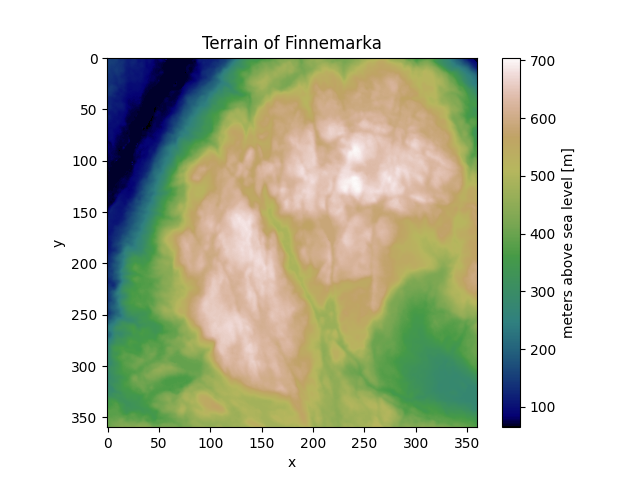
\includegraphics[width=\linewidth, height=7cm]{Figure20.png}
\caption{The Finnemark elevation dataset}
		\end{figure}

		\section{Methods}
%How did you obtain the data, what methods did you use? Describe your work process. If you performed an experiment using specific equipment, describe your setup.
			\subsection{Scaling}
It is useful to scale our data before we perform any approximation of our dataset, as this will help us to account for problems with outliers and particularly large values when we fit. We will use the simple standard scaling from \textit{Sklearn.preprocessing} called scale. This subtracts the mean value from the data points.

			\subsection{Building the Model}
When performing a linear regression, we want a model on the form
			\begin{equation}
z = \sum_{i = 0}^{p} \sum_{j = 0}^{i} \beta_{\sum_{k = 0}^{i} + j} x^{i - j}y^{j}
			\end{equation}
This might look odd, but is just a compact way of writing a standard 2 dimensional $p$ degree polynomial. for $p = 2$ this is simply
			\begin{equation*}
z = \beta_0 + \beta_1 x + \beta_2 y + \beta_3 x^2 + \beta_4 xy + \beta_5 y^2 
			\end{equation*}
To perform this regression we need to set up a matrix $X$ on the form
			\begin{equation}
\vec{X} = \left[ \begin{matrix}
\sum_{i = 0}^{p} \sum_{j = 0}^{i} x_0^{i - j}y_0^{j} \\
\sum_{i = 0}^{p} \sum_{j = 0}^{i} x_1^{i - j}y_1^{j} \\
\dots \\
\sum_{i = 0}^{p} \sum_{j = 0}^{i} x_n^{i - j}y_n^{j} \\
\end{matrix} \right]
			\end{equation}
where $n$ are the number of $x, y$ pairs in the dataset. \\
Then we can split our dataset into two groups, a training and a test group. We use $20\%$ of our dataset as a test and the rest as training group.

				\subsubsection{Ordinary Least Squares}
Now we are prepared to model our data with the OLS method. This is a simple task where we approximate the $\beta$ values by finding the minimum value of the cost function
				\begin{equation*}
C(\vec{\beta}) =  \frac{1}{n} \left\{ \left( \vec{y} - \vec{X} \vec{\beta} \right)^{T} \left( \vec{y} - \vec{X} \vec{\beta} \right) \right\}
				\end{equation*}
It is simple to show, by taking the derivative of $C$ that the minimum point can be found from
				\begin{equation}
\vec{\beta} = \left( \vec{X} \vec{X}^T \right)^{-1} \vec{X}^T \vec{y}
				\end{equation}
as long as $\vec{X} \vec{X}^T$ is transposable. If they are not, we can approximate them by the Moore-Penrose pseudo-inverse instead, and use this result.

			\subsubsection{Ridge Regression}
Another way to perform the Linear regression is the Ridge method. This is almost the same as the OLS, except the introduction of a constant $\lambda$ times the norm of $\beta$ into the cost function.
				\begin{equation*}
C(\vec{\beta}) =  \frac{1}{n} \left\{ \left( \vec{y} - \vec{X} \vec{\beta} \right)^{T} \left( \vec{y} - \vec{X} \vec{\beta} \right) \right\} + \lambda ||\beta||_2^2
				\end{equation*}
This gives us a way to find beta in the same way as for the OLS except with a $\lambda$ times an identity matrix
				\begin{equation}
\vec{\beta} = \left( \vec{X} \vec{X}^T + \lambda \vec{I} \right)^{-1} \vec{X}^T \vec{y}
				\end{equation}
With the same assumption as for the OLS.

			\subsubsection{Lasso Regression}
The last regression method is the Lasso regression, where we define the cost function to be equal to
				\begin{equation*}
C(\vec{\beta}) =  \frac{1}{n} \left\{ \left( \vec{y} - \vec{X} \vec{\beta} \right)^{T} \left( \vec{y} - \vec{X} \vec{\beta} \right) \right\} + \lambda ||\beta||_1
				\end{equation*}
where we have used $||\beta||_1 = \sum_{i} |\beta|$. This doesn't have a numerical solution to the derivative of $C$ like the other two methods. However, the python package \textit{sklearn} has a useful method \textit{linear\_model.Lasso} which we can use to perform this minimalisation task for us. \\

			\subsection{Analysis methods}
We need to find a way to measure which method is the best at approximating our dataset, and to do this a simple measure might be to look at the Mean Square Error and use this as our prediction error.
				\subsubsection{Mean Square Error}
The MSE is simply the mean value of the square of the errors between the approximations and the measured values.
				\begin{equation}
MSE = \frac{1}{n} \sum_{i} \left( z_i - \hat{z}_i \right)^2
				\end{equation}
where $z$ are the measured values and $\hat{z}$ are the true values. \\
				\subsubsection{R Squared}
We can also calculate the $R^2$ value of the model, which is defined as
				\begin{equation}
R^2 = 1 - \frac{\sum_{i} \left( z_i - \hat{z}_i \right)^2}{\sum_{i} \left( z_i - \bar{\hat{z}} \right)^2}
				\end{equation}
$\bar{\hat{z}}$ is the mean value of the approximations. \\
				\subsubsection{Bootstrap Resampling}
A more complicated, but still quite simple way to find the best fit model is to perform the bootstrap resampling method. This method is based on the assumption that we can perform the prediction of our data a number of times $a$, where we each time choose a random subset of the test and training group with replacing. Thus we get $a$ new train and test groups, with the same size as the original once, and we can find the MSE for each and averaging over all the MSEs. From this we can also split the MSE into three other parts, the Bias, the Variance and the variance of the error. To get this, we can look at the MSE
				\begin{align*}
MSE =& \frac{1}{n} \sum_{i} \left( z_i - \hat{z}_i \right)^2 \\
=& \text{E}\left[ \left( \vec{z} - \hat{\vec{z}} \right)^2 \right]
				\end{align*}
where E denotes the expected value. If we add $E[\hat{\vec{z}}] - E[\hat{\vec{z}}]$ inside the square and perform the squaring, we can rewrite this as 
				\begin{align*}
MSE =& \text{E}\left[ \left( \hat{\vec{z}} - E[\hat{\vec{z}}] \right)^2 \right. \\
&+ \left( \vec{z} - E[\hat{\vec{z}}] \right)^2 \\
&\left.+ 2 \left( E[\hat{\vec{z}}] - \vec{z} \right) \left( \hat{\vec{z}} - E[\hat{\vec{z}}] \right) \right]
				\end{align*}
The estimated value of an estimated value is simply the estimated value, and the estimated value of a measured value is simply the measured value. This lets us rewrite the above as
				\begin{align*}
MSE =& \text{E}\left[ \left( \hat{\vec{z}} - E[\hat{\vec{z}}] \right)^2 \right] \\
&+ E \left[ \left( \vec{z} - E[\hat{\vec{z}}] \right)^2 \right] \\
&+ 2 \left( E[\hat{\vec{z}}] - \vec{z} \right) \left( E[\hat{\vec{z}}] - E[\hat{\vec{z}}] \right) \\
=& \text{E}\left[ \left( \hat{\vec{z}} - E[\hat{\vec{z}}] \right)^2 \right] \\
&+ E \left[ \left( \vec{z} - E[\hat{\vec{z}}] \right)^2 \right] \\
=& \text{Var}(\hat{\vec{z}}) + \sigma^2 + \text{Bias}(\vec{z}, \hat{\vec{z}})^2
				\end{align*}
The Last step her is just splitting the left term into the variance of the model and the variance of the assumed noise. This result gives us the bias and the variance
				\begin{align}
\text{Bias} =& \frac{1}{n} \sum_i \left( z_i - E[\hat{\vec{z}}] \right)^2 \\
\text{Var} =& \frac{1}{n} \sum_i \left( \hat{\vec{z}} - E[\hat{\vec{z}}] \right)^2
				\end{align}
As we can see, the bias is simply the average of the difference between the measured value and the estimated approximation value. The Variance is the same, but the measured value is exchanged for the approximated value. \\

				\subsubsection{Cross Validation}
We can then calculate the MSE, bias and variance and plot them as a function of our polynomial degree, to find at what value the bias and variance has the optimal values. \\
Last of all, we can perform the so called Cross Validation resampling method (CV). Here we shuffle and perform a random split of data into test and training groups a number of times $N$ and calculate the MSE every time. Then we find the mean of this value and use this as our MSE estimate.

				\subsection{Performing the analysis}
First We will perform the analysis methods for OLS, finding the best fit polynomial degree. Then we will find the optimal lambda for Ridge and Lasso, using a degree of 5. This we do for the Franke function to test our method, afterwords we can perform the same thing for the terrain data. Last, we use this lambdas for the terrain data to find the optimal degree and compare the best fit models for OLS, Ridge and Lasso.

		\section{Results}
%What were your clear-cut results? - Present them in a clear and concise manner, waiting with the discussion of them for later. Here you present calculations, figures and tables of data, output of code, etc.
Performing the OLS estimate of the Franke dataset with a fifth degree polynomial, we get an $R^2$ value of $0.9927$ This also gives us the following visualisation of the approximation
			\begin{figure}[H]
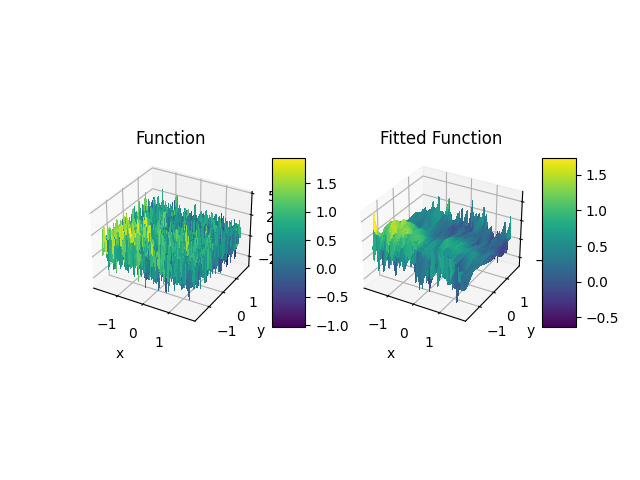
\includegraphics[width=\linewidth, height=7cm]{Figure10.png}
\caption{The Franke and the fitted approximation with OLS}
			\end{figure}
To the left in figure (2) we see the actual Franke function and to the right we see the 5th order approximation with OLS. \\
For the OLS we get a MSE as a function for the polynomial degree for both the training and test data.
			\begin{figure}[H]
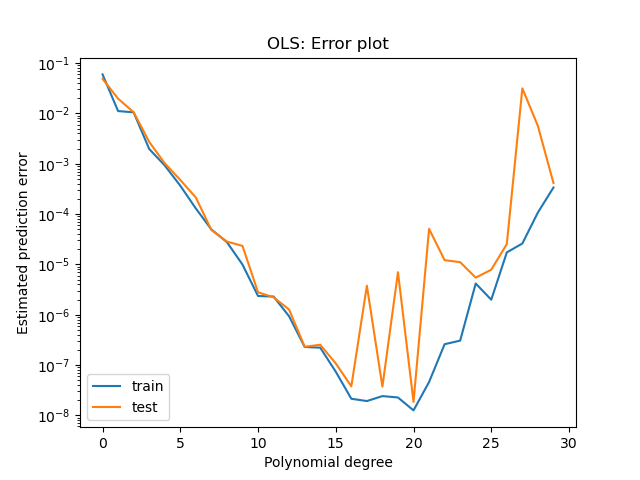
\includegraphics[width=\linewidth, height=7cm]{Figure01.png}
\caption{MSE as a function of polynomial degree for both the test and train data set groups}
			\end{figure}
We see that both dataset groups MSEs get reduced with higher polynomial degree until we reach around 20 and then they both rise up, but the test rises faster. \\
The Bootstrap for the OLS gives us a plot of the MSE, Bias and Variance.
			\begin{figure}[H]
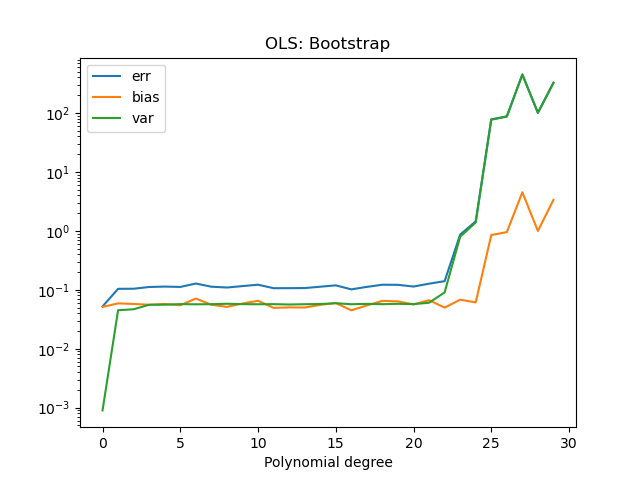
\includegraphics[width=\linewidth, height=7cm]{Figure02.png}
\caption{Bootstrap MSE, bias and variance for OLS. Rises in value after 20th degree.}
			\end{figure}
They all stay quite low until after 20th degree where they rise up. \\
The CV gives us a MSE which we can compare with the MSE of Bootstrap
			\begin{figure}[H]
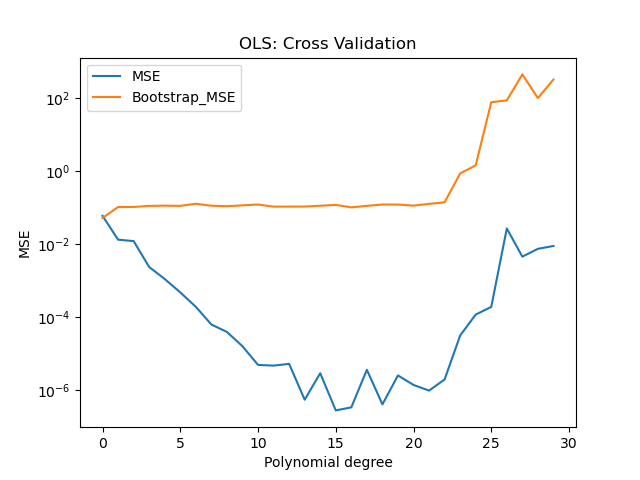
\includegraphics[width=\linewidth, height=7cm]{Figure03.png}
\caption{CV MSE estimate for OLS compared with the Bootstrap MSE. The CV has a minimum which the Bootstrap doesn't have}
			\end{figure}
We see that the CV gives us a minimum point that the Bootstrap didn't. \\
For the Ridge we get a MSE as a function for the lambda for both the training and test data
			\begin{figure}[H]
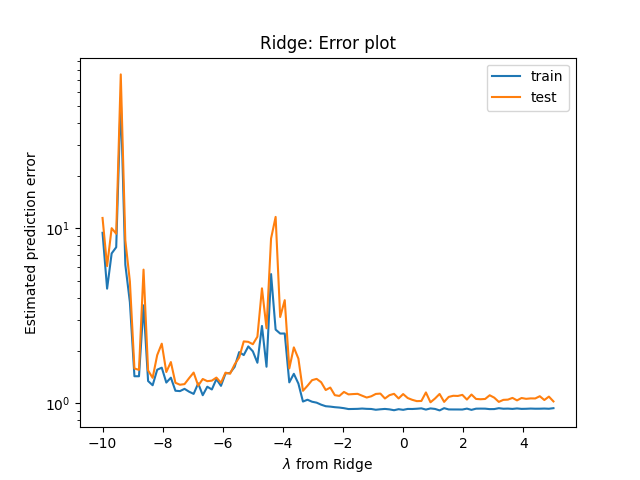
\includegraphics[width=\linewidth, height=7cm]{Figure04.png}
\caption{MSE as a function of lambda for both the test and train data set groups}
			\end{figure}
We see that both dataset groups MSEs look mostly the same. They fluctuate a little until they reach a minimum around zero and rise afterwards slowly up. \\
The Bootstrap for the Ridge gives us a plot of the MSE, Bias and Variance.
			\begin{figure}[H]
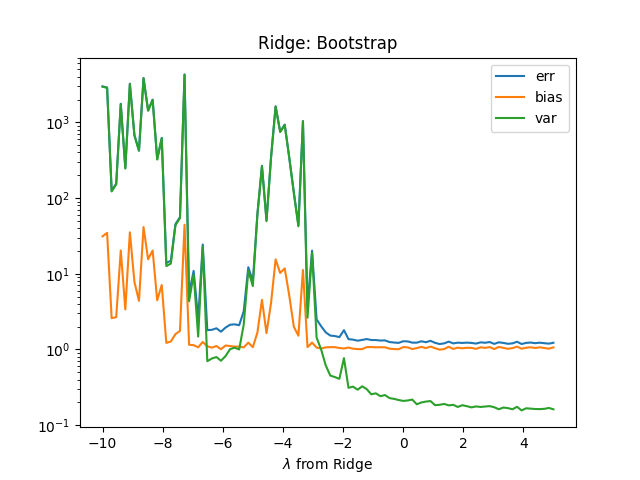
\includegraphics[width=\linewidth, height=7cm]{Figure05.png}
\caption{Bootstrap MSE, bias and variance for Ridge. After lambda equal to zero they all stabilise at a low value.}
			\end{figure}
We see all three quantities fluctuate for negative values of lambda, but stabilise after zero for quite a low value. \\
The CV gives us a MSE which we can compare with the MSE of Bootstrap
			\begin{figure}[H]
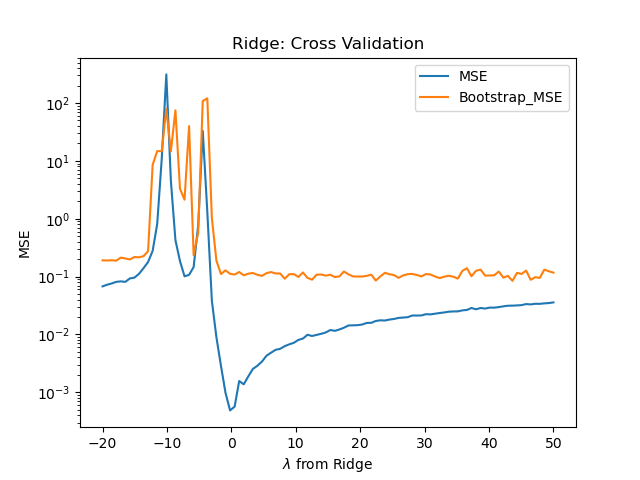
\includegraphics[width=\linewidth, height=7cm]{Figure06.png}
\caption{CV MSE estimate for Ridge compared with the Bootstrap MSE. The CV has a minimum which the Bootstrap doesn't have}
			\end{figure}
We see that the CV gives us a minimum point that the Bootstrap didn't at lambda around zero. but it doesn't stabilise after zero but rather looks like it converges to the same value as Bootstrap for some very high lambda. \\
For the Lasso we get a MSE as a function for the polynomial degree for both the training and test data.
			\begin{figure}[H]
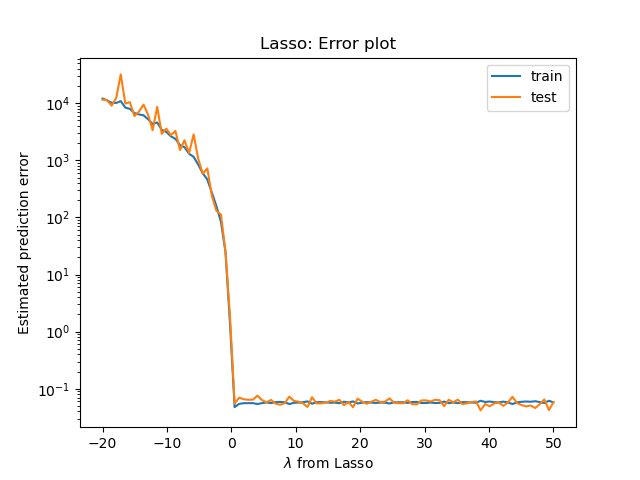
\includegraphics[width=\linewidth, height=7cm]{Figure07.png}
\caption{MSE as a function of lambda for both the test and train data set groups}
			\end{figure}
We see that both dataset groups have the same evolution, falling down at zero and staying the same after this \\
The Bootstrap for the Lasso gives us a plot of the MSE, Bias and Variance.
			\begin{figure}[H]
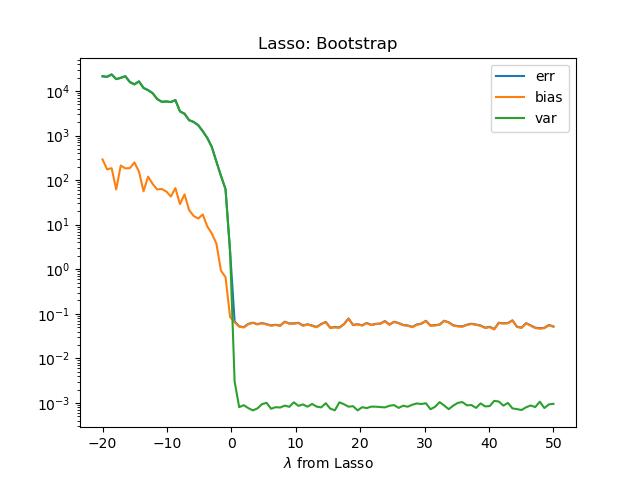
\includegraphics[width=\linewidth, height=7cm]{Figure08.png}
\caption{Bootstrap MSE, bias and variance for Lasso. Has the same general form as the error plot, but we can't see the error because it follows the other values so much.}
			\end{figure}
Varians starts high but drop off a lot at zero. Until then, the error follows this. Then, at lambda equal to zero, the bias passes the variance and the error starts following this. \\
The CV gives us a MSE which we can compare with the MSE of Bootstrap
			\begin{figure}[H]
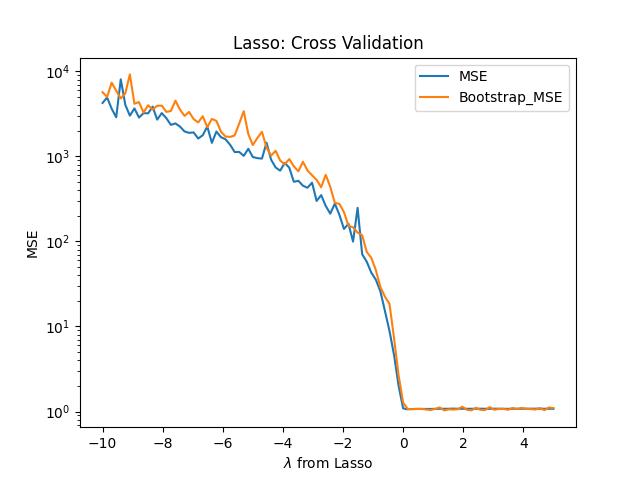
\includegraphics[width=\linewidth, height=7cm]{Figure09.png}
\caption{CV MSE estimate for Lasso compared with the Bootstrap MSE. The CV and Bootstrap look the same.}
			\end{figure}
We see that the CV and Bootstrap gives us the same form. \\
For the OLS we get the following analysis plots
			\begin{figure}[H]
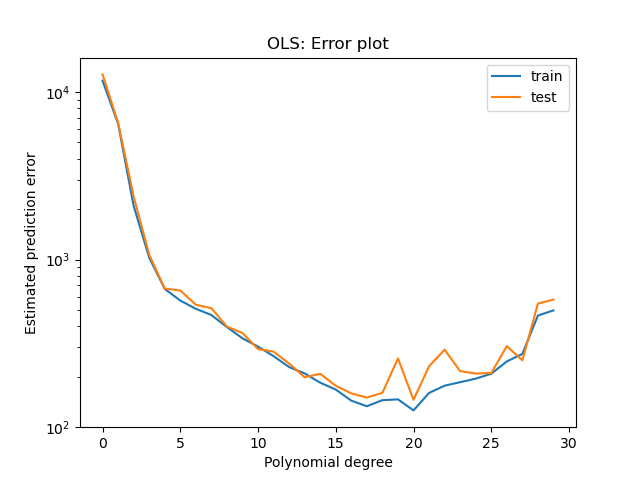
\includegraphics[width=\linewidth, height=7cm]{Figure11.png}
\caption{MSE for OLS for both training and test groups with the terrain data set}
			\end{figure}
			\begin{figure}[H]
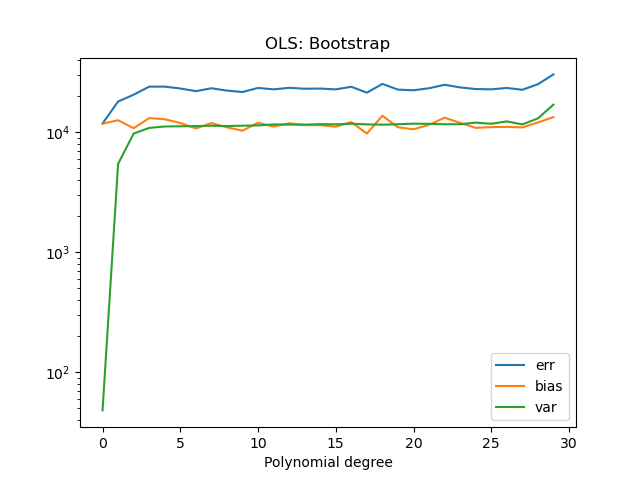
\includegraphics[width=\linewidth, height=7cm]{Figure12.png}
\caption{MSE, Bias and Variance for OLS with the terrain data set}
			\end{figure}
			\begin{figure}[H]
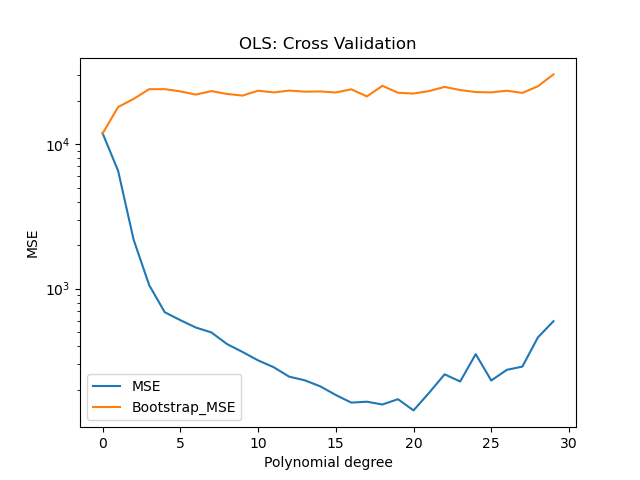
\includegraphics[width=\linewidth, height=7cm]{Figure13.png}
\caption{MSE for OLS for both CV and Bootstrap with the terrain data set}
			\end{figure}
We see that all three plots gives us a minimum at around the same polynomial degree, though the Bootstrap result is almost constant for all polynomial degrees. \\
For the Ridge we get the following analysis plots
			\begin{figure}[H]
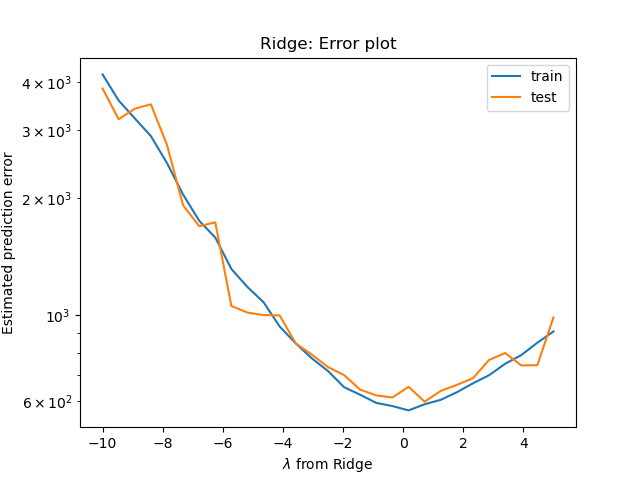
\includegraphics[width=\linewidth, height=7cm]{Figure14.png}
\caption{MSE for Ridge for both training and test groups with the terrain data set}
			\end{figure}
			\begin{figure}[H]
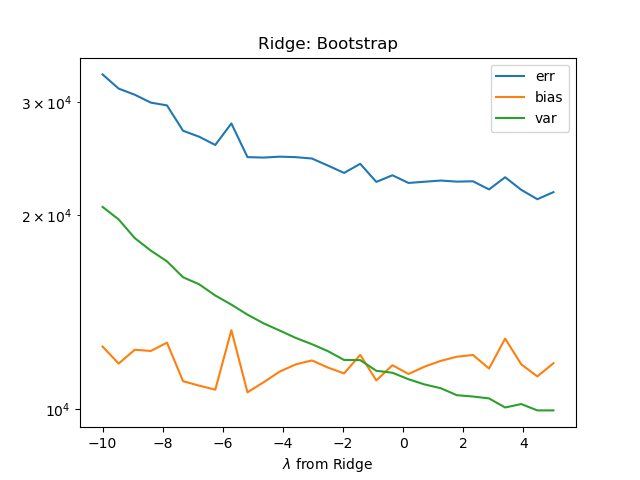
\includegraphics[width=\linewidth, height=7cm]{Figure15.png}
\caption{MSE, Bias and Variance for Ridge with the terrain data set}
			\end{figure}
			\begin{figure}[H]
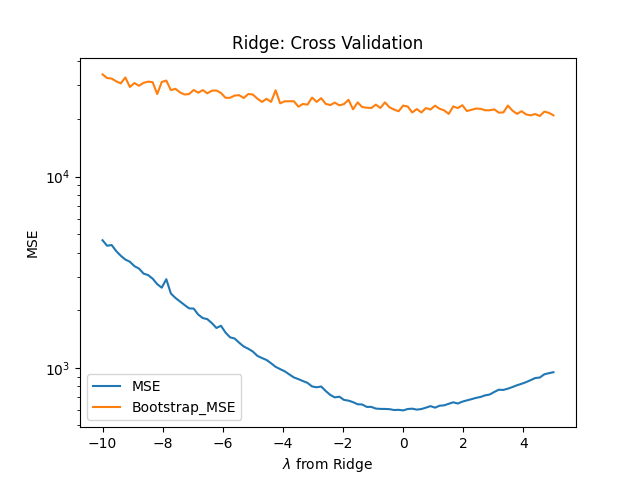
\includegraphics[width=\linewidth, height=7cm]{Figure16.png}
\caption{MSE for Ridge for both CV and Bootstrap with the terrain data set}
			\end{figure}
We see that the error and CV gives us a minimum lambda value, but the Bootstraps just drops of for rising values. \\
For the Lasso we get the following analysis plots
			\begin{figure}[H]
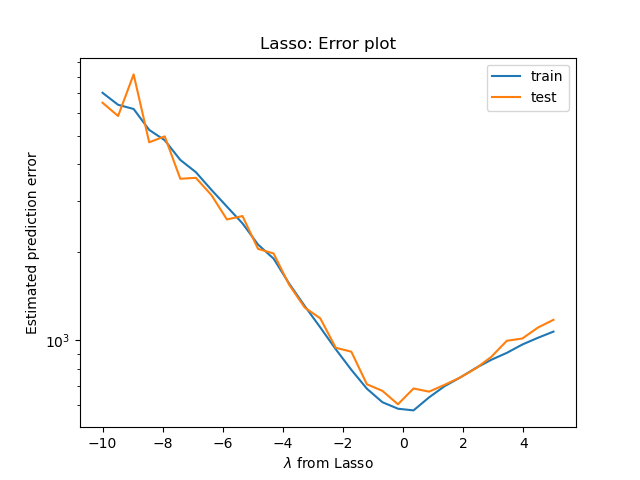
\includegraphics[width=\linewidth, height=7cm]{Figure17.png}
\caption{MSE for Lasso for both training and test groups with the terrain data set}
			\end{figure}
			\begin{figure}[H]
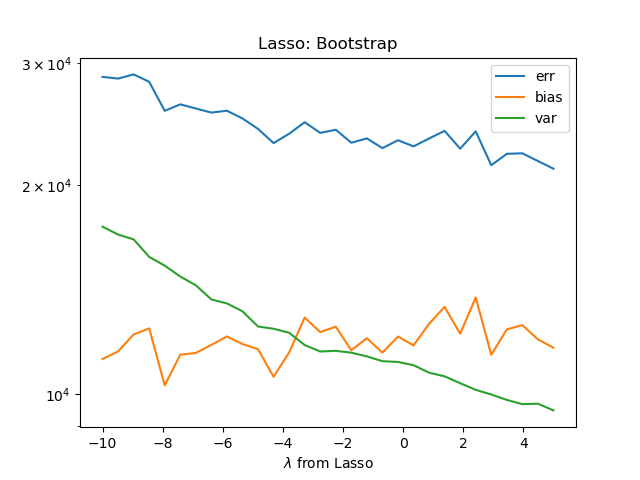
\includegraphics[width=\linewidth, height=7cm]{Figure18.png}
\caption{MSE, Bias and Variance for Lasso with the terrain data set}
			\end{figure}
			\begin{figure}[H]
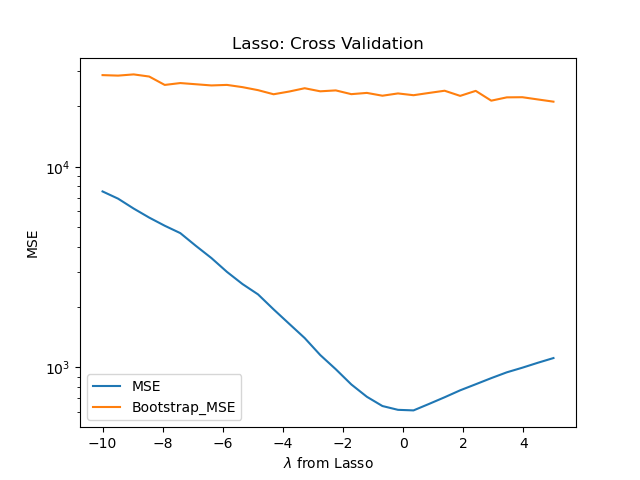
\includegraphics[width=\linewidth, height=7cm]{Figure19.png}
\caption{MSE for Lasso for both CV and Bootstrap with the terrain data set}
			\end{figure}
We see that the error and CV gives us a minimum lambda value, but the Bootstraps just drops of for rising values just like we saw for Ridge. \\
Using these optimal values, we get the following analysis plots for Ridge as functions of polynomial degree.
			\begin{figure}[H]
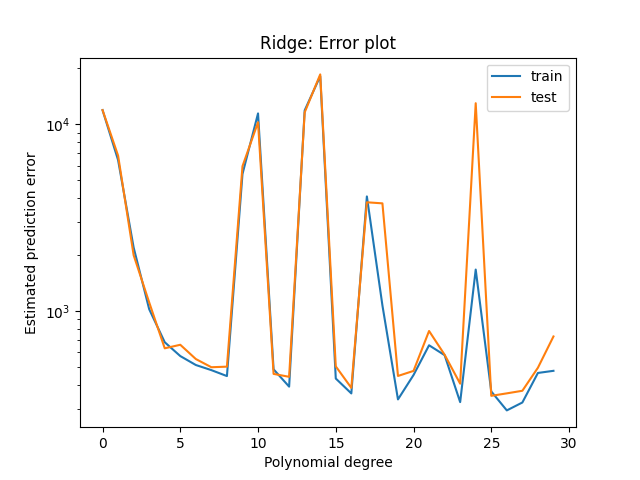
\includegraphics[width=\linewidth, height=7cm]{Figure21.png}
\caption{MSE for Ridge for both training and test groups with the terrain data set as a function of polynomial degree}
			\end{figure}
			\begin{figure}[H]
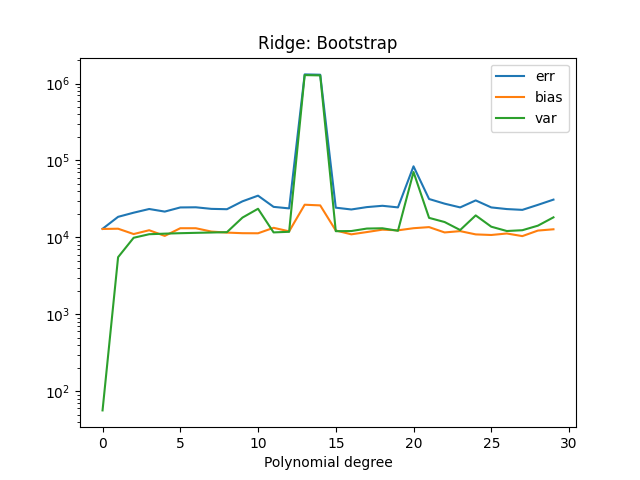
\includegraphics[width=\linewidth, height=7cm]{Figure22.png}
\caption{MSE, Bias and Variance for Ridge with the terrain data set as a function of polynomial degree}
			\end{figure}
			\begin{figure}[H]
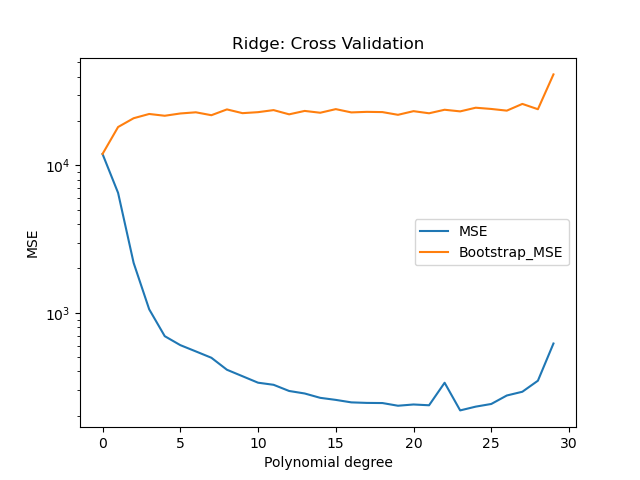
\includegraphics[width=\linewidth, height=7cm]{Figure23.png}
\caption{MSE for Ridge for both CV and Bootstrap with the terrain data set as a function of polynomial degree}
			\end{figure}
We see that the error and CV gives us a minimum lambda value, but the Bootstraps stay constant for most of the plot. \\
For the optimal models we get the following estimated errors \\
			\begin{tabular}{|l|c|c|}
\hline
& OLS & Ridge \\
\hline
MSE & 188.6160408 & 227.8683254 \\
Bootstrap MSE & 28119.19033 & 24358.41955 \\
CV MSE & 157.1029735 & 225.2837576 \\
\hline
			\end{tabular}

		\section{Discussion}
%Were the results what you expected? Are the results significant? - meaning; are the results clear, or are they open to interpretation? How certain can you be of them? What do these results mean in a wider context?
From the analysis of the Franke function we can see that all the different methods have a best fit value and in the error plots. However, the bootstrap results are odd for every regression method. Though the mean square error looks like it is the sum of the variance and the bias like we would expect, the variance follows the same evolution of the bias, instead of being the opposite like we would expect. As for the Cross Validation we see about the same evolution as the Error. As for the terrain data, we see almost the same things as for the Franke function, but we can still use the MSE and the CV to find an optimal lambda and polynomial degree. We find $p = 20$ as the optimal for OLS, $\lambda = 0.1$ and $p = 23$ for the Ridge and $\lambda = 0.2$ for the Lasso. However, for the Lasso regression, with the best fit lambda we couldn't get the Lasso regression to converge into a best fit, making this method unavailable. From the calculations of the errors of these best fits, we have that the OLS gives the best fit for our dataset. \\
A problem we have overlooked in this analysis is that we have not calculated confidence interval. This would have been a simple task, but I didn't have the time to do so. \\
Another problem is that we have chosen to perform the estimation of lambda first, and then the estimation of polynomial degree for the Ridge and Lasso. This was done to save time, as the calculations where very time consuming.

		\section{Conclusion}
We saw that all the methods estimate a best fit for the Franke function, and for the terrain data, except that the Lasso doesn't converge for the polynomial degree. However we get a best fit for the other two, and from our best fit models we end up with the model best fitting our terrain data is the Ordinary Least Squares model of a $20$th degree polynomial.
		
\addcontentsline{toc}{section}{Bibliography}
		\begin{thebibliography}{9}
%			\bibitem{<Name of referance>}
%<Name of Author, Name of Author, ...>; \\
%<Title of article> \\
%\url{<URL>} \\
%<Published Date of release> \\
%<Downloaded Date you downloaded webpage>
%			\bibitem{<Name of referance>}
%<Name of Author, Name of Author, ...>; \\
%<Title of article>, <Pages used> \\
%<Year of release>, <Town published>: <Publisher> \\
			\bibitem{USGS}
United States Geological Survey; \\
Earth explorer \\
\url{https://earthexplorer.usgs.gov/} \\
Published 23/09-2014 \\
Downloaded 10/10-2020
		\end{thebibliography}
	\end{multicols}
\end{document}